% Phase 1 deck. Build: cd slides && tectonic slides.tex  ->  slides/slides.pdf
% Figures come from ../reports/figures/ only. Slide owners are noted above each frame.
\documentclass[aspectratio=169,11pt]{beamer}
\usepackage{booktabs}
\usepackage{array}
\usepackage{amsmath}

\definecolor{accent}{HTML}{3D5A80}
\definecolor{muted}{HTML}{5C6670}
\definecolor{tblhead}{HTML}{E9ECEF}

\setbeamercolor{frametitle}{fg=accent}
\setbeamercolor{title}{fg=accent}
\setbeamercolor{structure}{fg=accent}
\setbeamercolor{normal text}{fg=black!85}
\setbeamerfont{frametitle}{size=\Large,series=\bfseries}
\setbeamertemplate{navigation symbols}{}
\setbeamertemplate{itemize items}{\small\raisebox{0.15ex}{$\bullet$}}
\setbeamertemplate{frametitle}{\vspace{0.6em}\insertframetitle\par\vspace{-0.2em}%
  {\color{accent}\rule{2.2cm}{1.2pt}}\par}
\setbeamertemplate{footline}{\hfill{\scriptsize\color{muted}\insertframenumber\,/\,\inserttotalframenumber}\hspace{1.2em}\vspace{0.8em}}
\setlength{\leftmargini}{1.1em}
\graphicspath{{../reports/figures/}}

\newcommand{\src}[1]{\par\vfill{\scriptsize\color{muted}#1}}

\title{Next Day Wildfire Spread Prediction}
\subtitle{Phase 1: per-pixel boosted trees with engineered spatial features}
\author{Harshil \and Sushant \and Priyanshu \and Sachin \and Piyush}
\institute{AML course project \quad CS \& AI Department, Rishihood University}
\date{}

\begin{document}

% ---------------------------------------------------------------- Piyush
\begin{frame}[plain]
\vfill
{\color{accent}\Huge\bfseries Next Day Wildfire Spread\\[0.2em] Prediction\par}
\vspace{0.6em}
{\large Phase 1: per-pixel boosted trees with engineered spatial features\par}
\vspace{0.4em}
{\color{accent}\rule{3cm}{1.5pt}\par}
\vspace{1.2em}
Harshil \quad Sushant \quad Priyanshu \quad Sachin \quad Piyush\par
\vspace{0.3em}
{\small\color{muted}AML course project \quad CS \& AI Department, Rishihood University\par}
\vfill
\end{frame}

% ---------------------------------------------------------------- Piyush
\begin{frame}{Problem: which pixels burn tomorrow?}
\begin{columns}[T]
\column{0.5\textwidth}
\small
\begin{itemize}
\item Input: 12 channels on day $t$ for a $64\times64$\,km patch at 1\,km (weather, terrain, vegetation, population, today's fire)
\item Output: probability that each pixel burns on day $t{+}1$
\item Fire is rare: 1.25\% of test pixels (1 in 80); cloud/smoke pixels ($-1$) are ignored
\item Accuracy fails: ``always no fire'' scores 98.7\%, our model 97.3\%. So we use \textbf{PR AUC}: precision vs recall on the fire class over all thresholds (random model = 0.0125, the fire rate)
\end{itemize}
\column{0.46\textwidth}
\centering
\vspace{2.5em}
\footnotesize
\begin{tabular}{@{}l r r@{}}
\toprule
Model & Accuracy & Fire found \\
\midrule
Always ``no fire'' & 98.7\% & 0\% \\
Our tuned XGBoost & 97.3\% & 53\% \\
\bottomrule
\end{tabular}
\end{columns}
\end{frame}

% ---------------------------------------------------------------- Priyanshu
\begin{frame}{Related work at a glance}
\begin{itemize}
\item Huot et al.\ 2022 built our dataset: pixel models up to 0.225 PR AUC, whole-patch CNN 0.284
\item Zhou et al.\ 2025: XGBoost on raw pixels only 0.06 PR AUC. Features, not the algorithm, decide what trees can do
\item Other papers use different crops, labels or metrics, so their scores are context only
\end{itemize}
\vspace{0.3em}
\centering
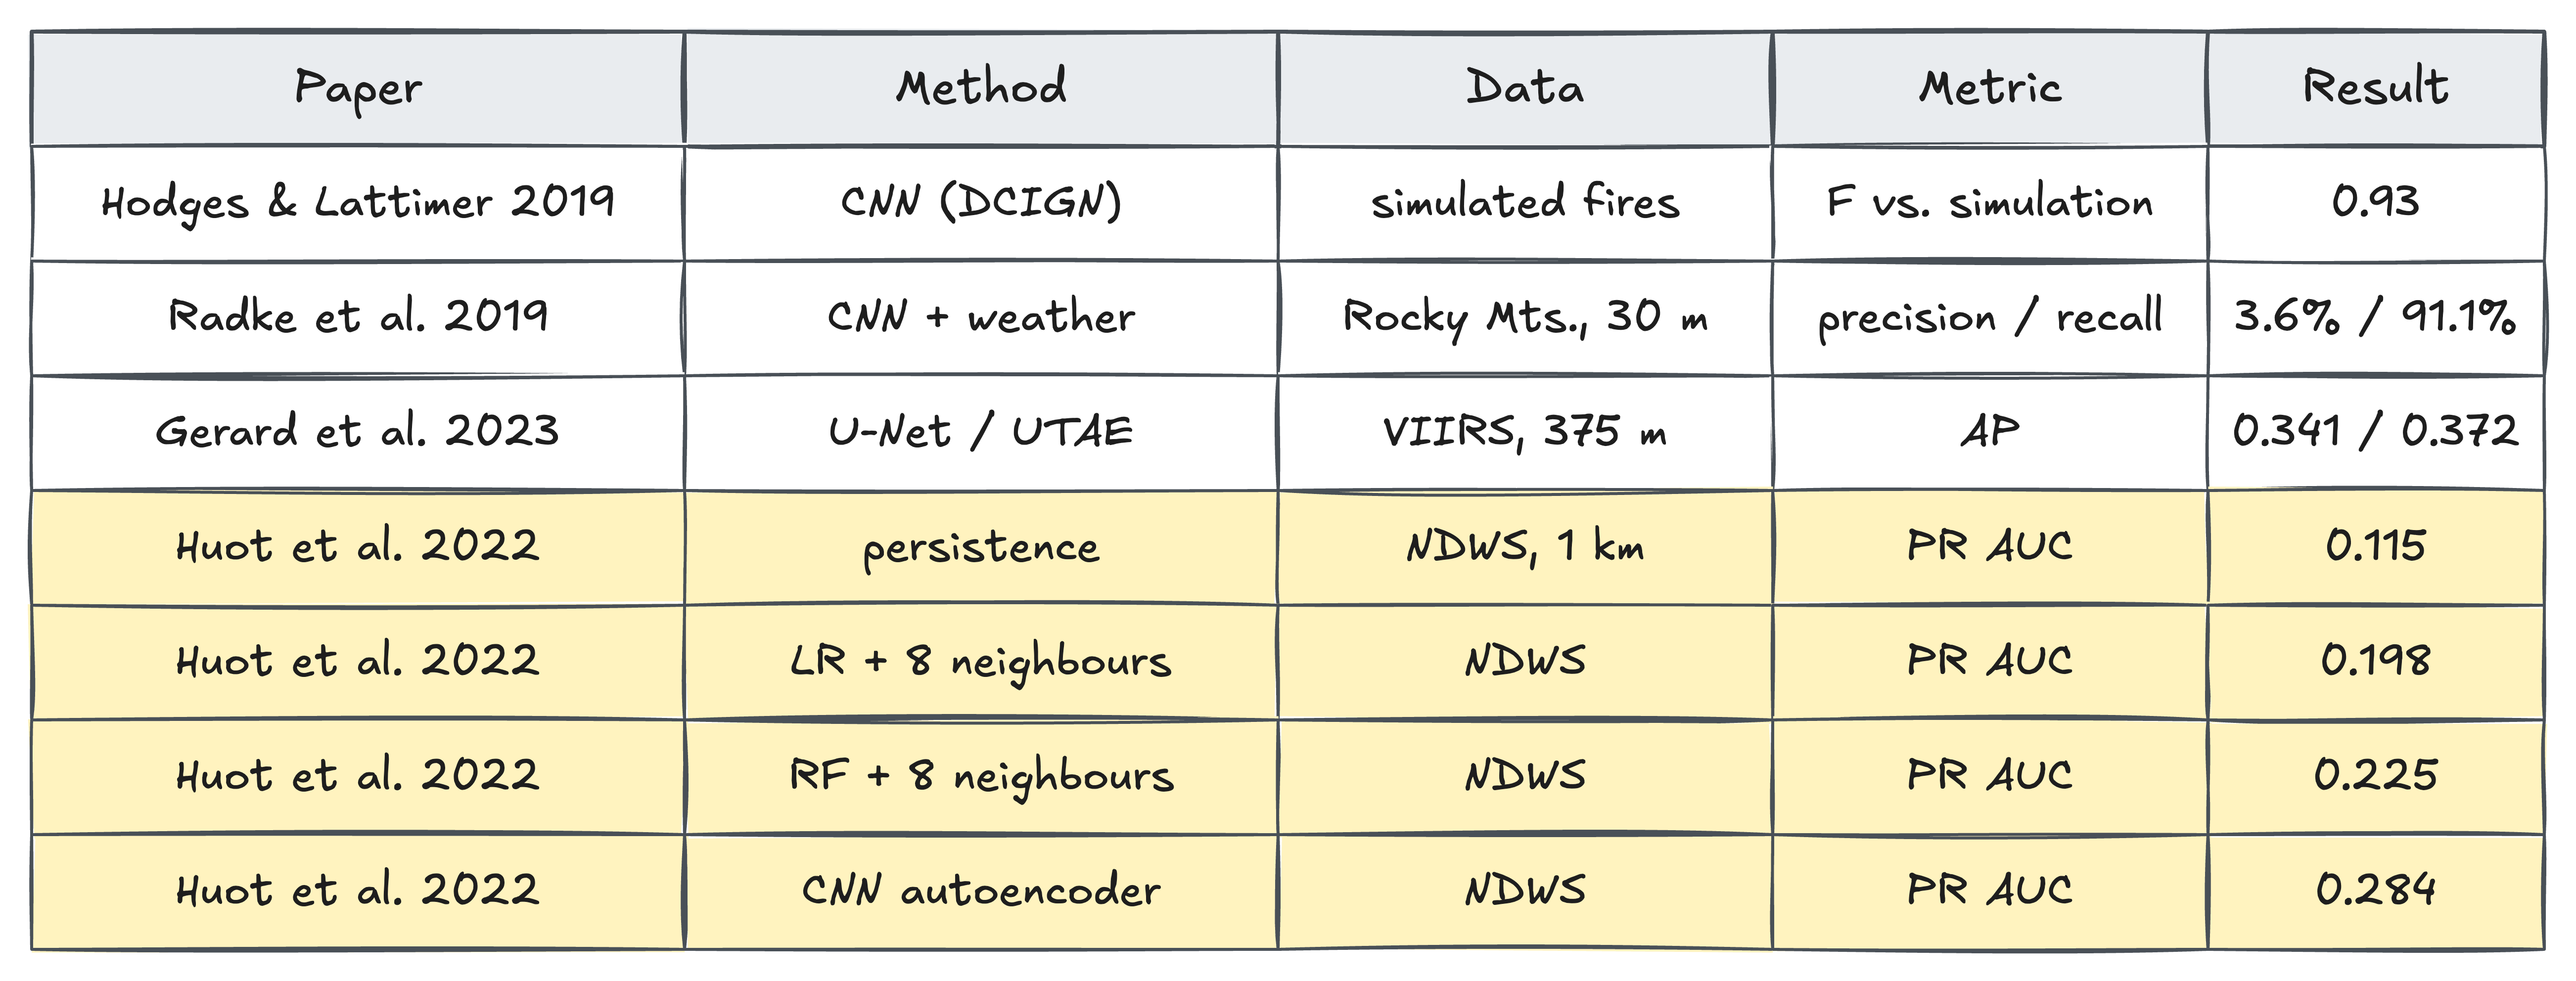
\includegraphics[width=0.7\textwidth]{slide1_related_work_table.png}
\end{frame}

% ---------------------------------------------------------------- Sushant
\begin{frame}{The dataset}
\begin{itemize}
\item 18\,545 patches of US fires (2012--2020); split by calendar week 8:1:1 $\rightarrow$ 14\,979 / 1\,877 / 1\,689
\item Labels: 1 fire, 0 no fire, $-1$ unknown (2.3--2.8\% of labels) $\rightarrow$ dropped from training and metrics
\item Fires change overnight: 58\% grow, 39\% shrink (train). Persistence misses growth and over-predicts shrinkage
\end{itemize}
\centering
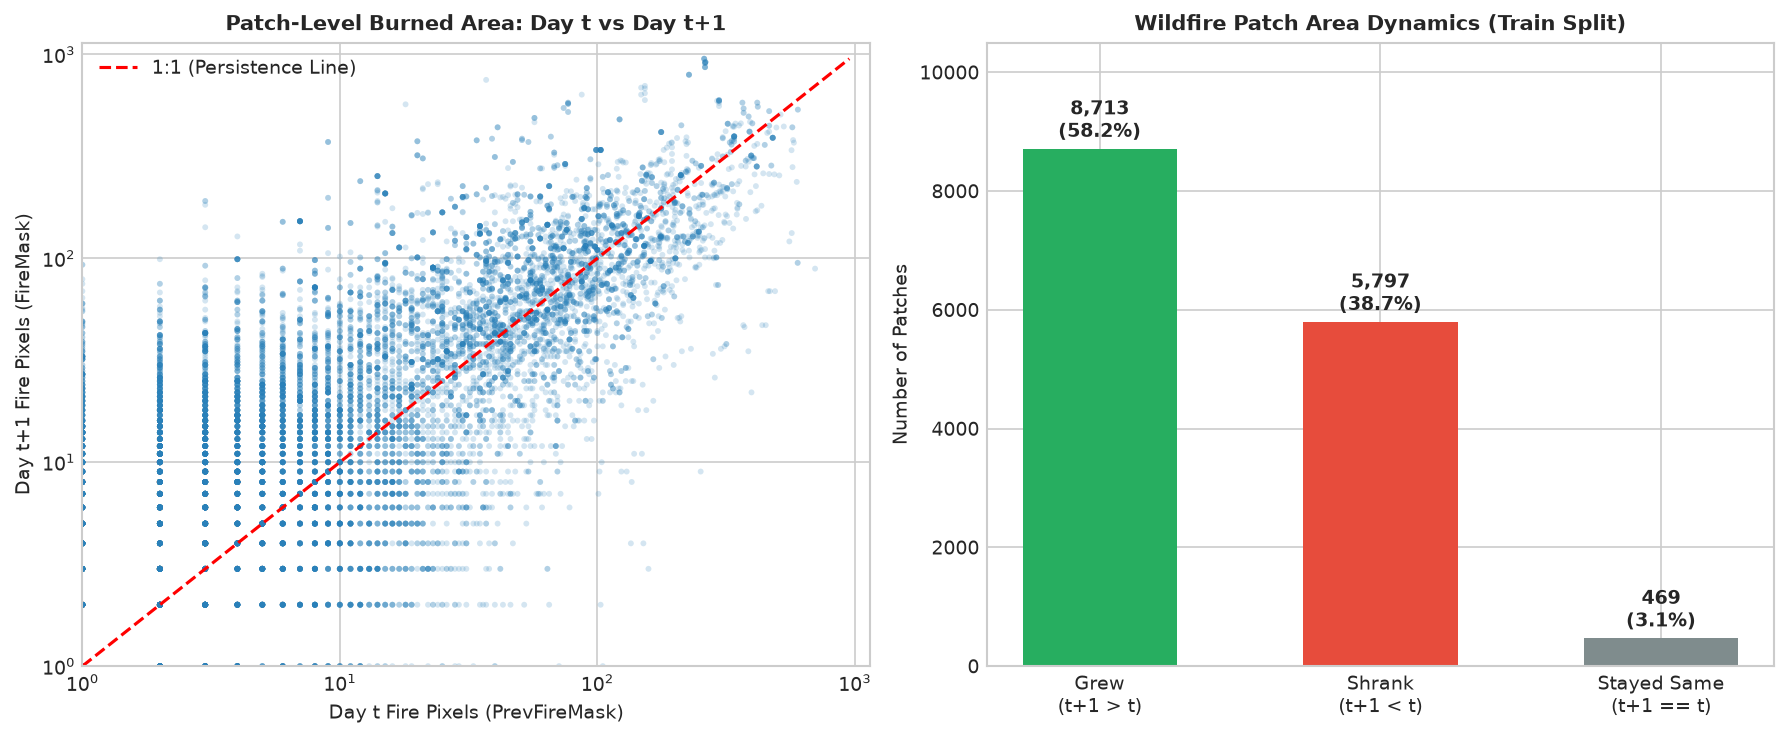
\includegraphics[width=0.56\textwidth]{eda_patch_fire_growth.png}
\src{Burned area per train patch on day $t$ vs $t{+}1$; dashed line = persistence.}
\end{frame}

% ---------------------------------------------------------------- Sushant + Harshil
\begin{frame}{Data traps: artefacts and a south-up grid}
\begin{columns}[T]
\column{0.46\textwidth}
{\color{accent}\bfseries Export artefacts}
\footnotesize
\begin{itemize}
\item Wind direction from $-505\,870^\circ$ to $37\,736^\circ$ $\rightarrow$ wrapped ($\theta \bmod 360$)
\item Temperatures from $-445$\,K to 1\,230\,K $\rightarrow$ clipped to $[253, 330]$\,K
\item Negative rain in 9.8\% of pixels $\rightarrow$ clipped to $\geq 0$
\item Bounds are physical constants, not fitted on data $\rightarrow$ no leakage
\end{itemize}
\column{0.5\textwidth}
{\color{accent}\bfseries Patches are stored south-up (not documented)}
\footnotesize
\begin{itemize}
\item North-facing slopes are greener in the Northern Hemisphere: slopes facing the last row have NDVI 0.596 vs 0.555 $\rightarrow$ the last row is north
\item Downwind/upwind next-day fire ratio at $\geq$ 8\,m/s: 3.1 with south-up, 0.37 with north-up (fire spreading into the wind is impossible)
\item Every wind feature depends on it: one constant, \texttt{ROW\_TO\_NORTH = 1}
\end{itemize}
\vspace{0.2em}
\centering
\footnotesize
\begin{tabular}{@{}l r@{}}
\toprule
Assumed orientation & Strong-wind ratio \\
\midrule
North-up & 0.37 \\
South-up & 3.1 \\
\bottomrule
\end{tabular}
\end{columns}
\src{Found because our first downwind check gave a physically impossible answer.}
\end{frame}

% ---------------------------------------------------------------- Piyush (from paper/sections/methodology.tex)
\begin{frame}{Method: from TFRecords to a per-pixel model}
\centering
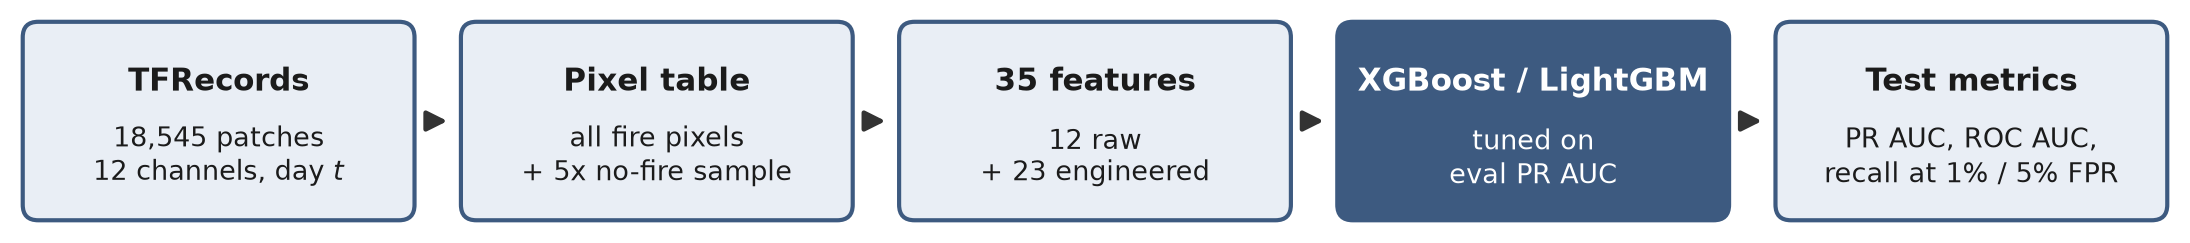
\includegraphics[width=\textwidth]{pipeline.png}
\vspace{0.6em}
\begin{columns}[T]
\column{0.49\textwidth}
\begin{itemize}
\item TFRecords parsed without TensorFlow into $(N,12,64,64)$ arrays
\item Artefacts clipped to fixed physical bounds; wind direction wrapped ($\theta \bmod 360$)
\item South-up orientation used by every direction feature (slide 5)
\end{itemize}
\column{0.49\textwidth}
\begin{itemize}
\item Training table: every fire pixel + 5:1 no-fire sample = 3.95\,M rows; \texttt{scale\_pos\_weight} = 5
\item 20 random configurations per model, early stopping on eval, best by eval PR AUC
\item Decision threshold: best F1 on eval, applied unchanged to test
\end{itemize}
\end{columns}
\end{frame}

% ---------------------------------------------------------------- Piyush (from paper/sections/methodology.tex)
\begin{frame}{Features: 12 raw + 23 engineered, in five groups}
\begin{columns}[T]
\column{0.56\textwidth}
\footnotesize
\begin{tabular}{@{}l r >{\raggedright\arraybackslash}p{3.7cm}@{}}
\toprule
Group & \# & Engineered examples \\
\midrule
Fire neighbourhood & 10 & fire density (3/5/9\,px), distance, fire upwind \\
Weather & 14 & wind $u$/$v$, VPD, min.\ rel.\ humidity, ERC $\times$ wind \\
Vegetation & 4 & local NDVI mean, std, anomaly \\
Terrain & 5 & slope, aspect, relative elevation \\
Human & 2 & population, $9\times9$ mean \\
\bottomrule
\end{tabular}
\vspace{0.2em}
\footnotesize
\begin{itemize}
\item \texttt{dist\_to\_fire}: univariate AUC 0.866 vs 0.593 for the raw fire mask
\item Most XGBoost gain is in fire features: \texttt{dist\_to\_fire} 32\%, \texttt{prev\_fire\_n9} 23\%, upwind 13.5\%
\end{itemize}
\column{0.42\textwidth}
\centering
\vspace{0.3em}
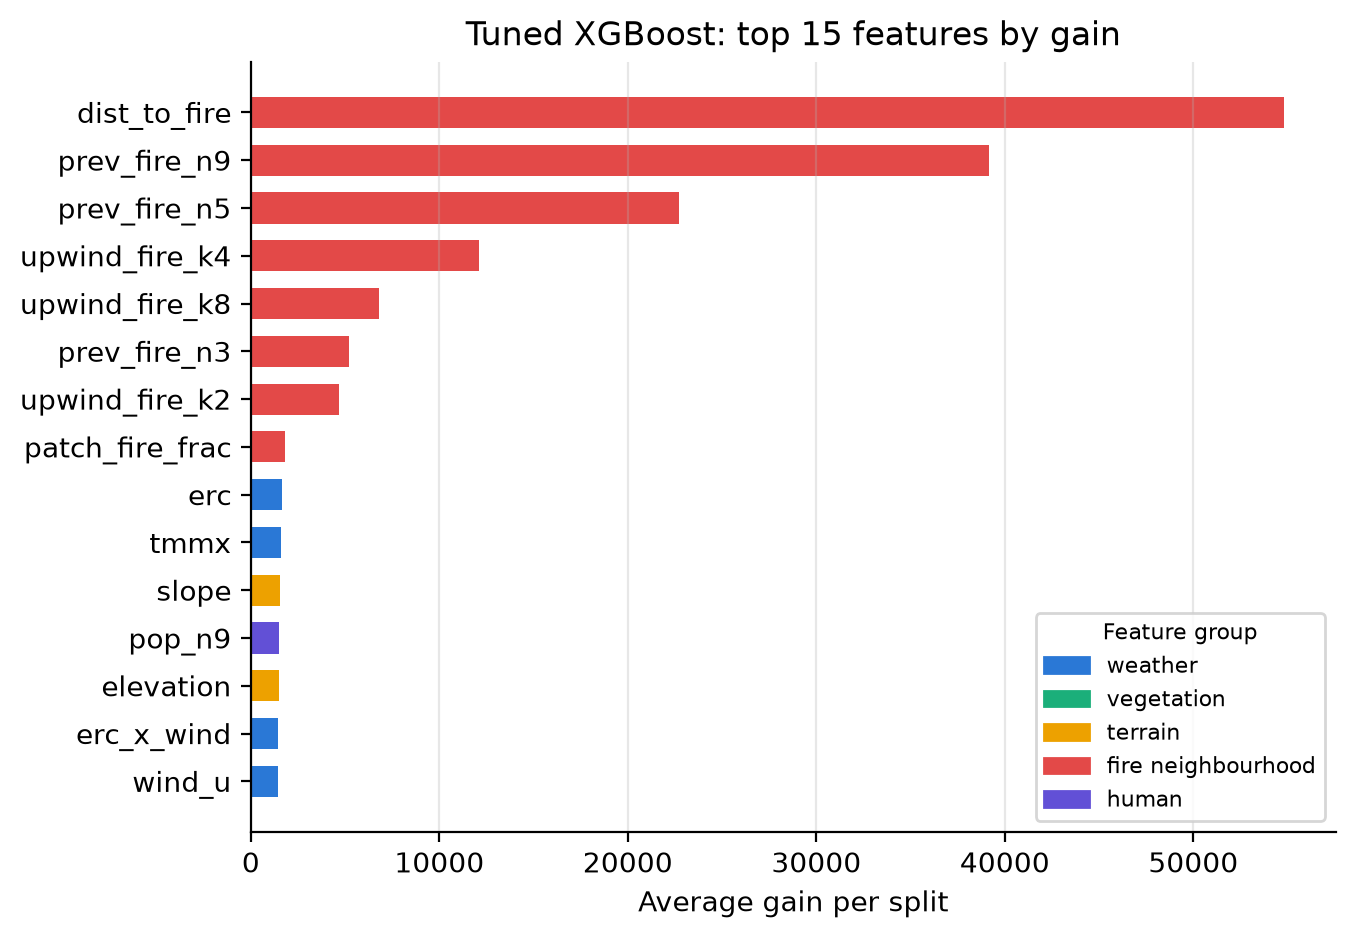
\includegraphics[width=\textwidth]{eval_gain_importance.png}
\end{columns}
\end{frame}

% ---------------------------------------------------------------- Sushant
\begin{frame}{From EDA to features, and what each group is worth}
\begin{columns}[T]
\column{0.44\textwidth}
\begin{itemize}
\item 40\% of new fire is more than 5\,km from day-$t$ fire $\rightarrow$ added \texttt{upwind\_fire\_k8} (ranks 5th of 35 by XGBoost gain)
\item Ablation: dropping fire-neighbourhood features drops PR AUC 0.248 $\rightarrow$ 0.048; vegetation is the most useful environmental group ($-0.009$)
\item Fire features alone: 0.218; environment adds $+0.031$ on top
\end{itemize}
\column{0.54\textwidth}
\centering
\vspace{0.5em}
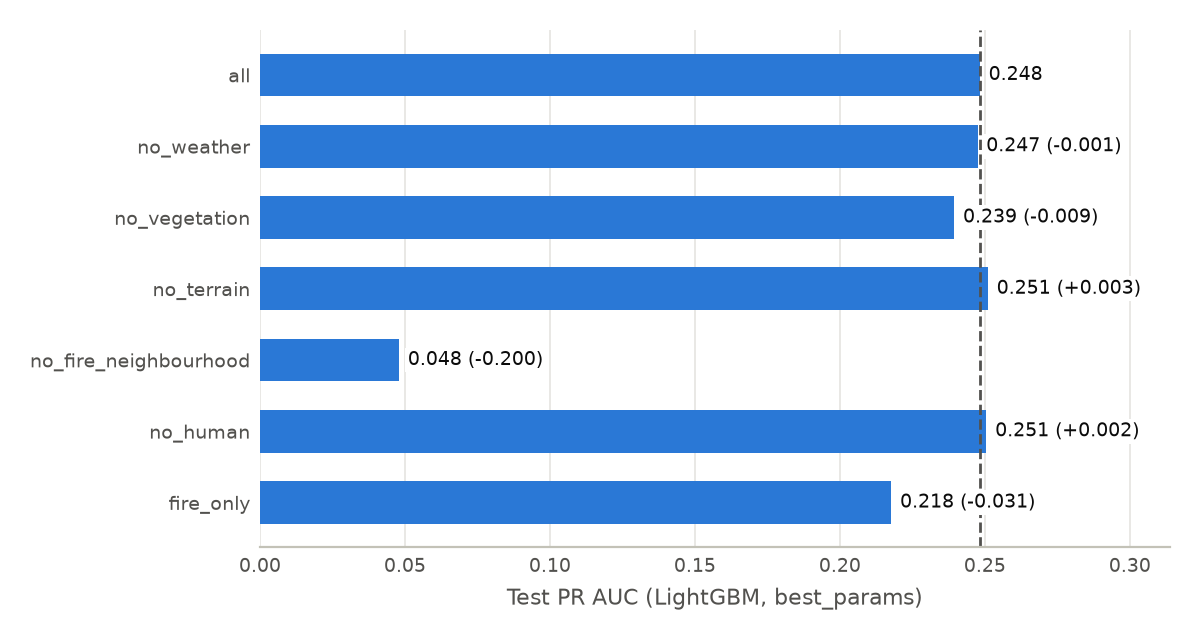
\includegraphics[width=\textwidth]{ablation_pr_auc.png}
\end{columns}
\end{frame}

% ---------------------------------------------------------------- Sachin
\begin{frame}{Results: same algorithm, nearly double the score}
\begin{columns}[T]
\column{0.64\textwidth}
\footnotesize
\setlength{\tabcolsep}{3pt}
\begin{tabular}{@{}l r r r r@{}}
\toprule
Model & PR AUC & ROC AUC & Recall & F1 \\
\midrule
Persistence & 0.106 & 0.633 & 0.273 & 0.309 \\
Logistic regression (raw) & 0.146 & 0.798 & 0.266 & 0.312 \\
Random forest (raw) & 0.157 & 0.816 & 0.270 & 0.312 \\
XGBoost (raw) & 0.145 & 0.795 & 0.257 & 0.292 \\
\textbf{XGBoost (tuned, 35 feat.)} & \textbf{0.257} & \textbf{0.906} & \textbf{0.526} & \textbf{0.332} \\
LightGBM (tuned, 35 feat.) & 0.248 & 0.903 & 0.520 & 0.331 \\
\bottomrule
\end{tabular}
\vspace{0.4em}
\small
\begin{itemize}
\item XGBoost raw 0.145 $\rightarrow$ with our features 0.257: the gain comes from the features
\item Recall doubles (26--27\% $\rightarrow$ 53\%) at 24\% precision; 39\% of fire found at 1\% FPR, 68\% at 5\% FPR
\end{itemize}
\column{0.34\textwidth}
\centering
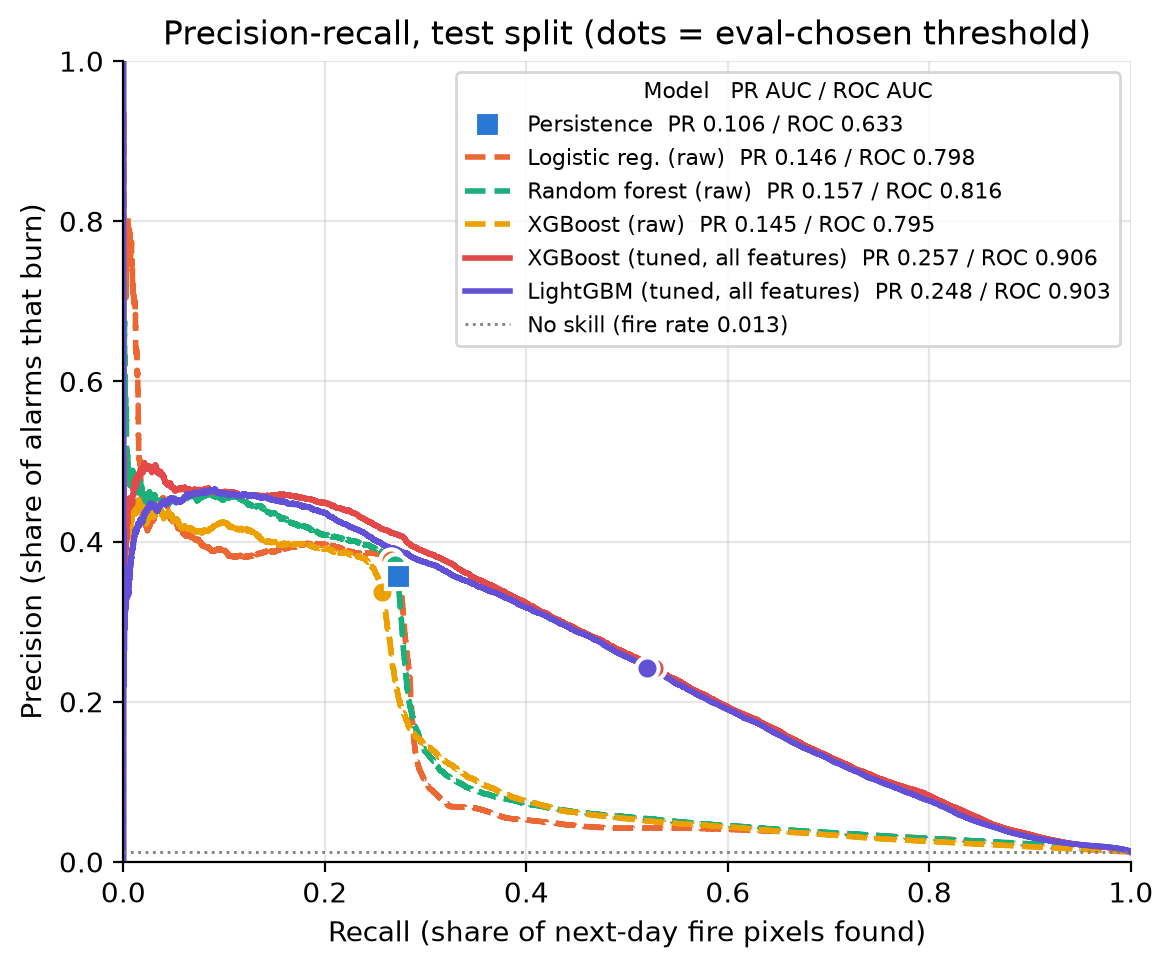
\includegraphics[width=\textwidth]{eval_pr_curves.png}
\end{columns}
\src{Test split; recall and F1 at the threshold chosen on eval.}
\end{frame}

% ---------------------------------------------------------------- Priyanshu
\begin{frame}{Where we stand}
\small
\begin{itemize}
\item 0.257 PR AUC; 95\% interval over fire events 0.19--0.33
\item Huot's RF (0.225) and CNN (0.284) both lie inside it $\rightarrow$ we sit between them, with no claim of being better
\item Raw XGBoost elsewhere: 0.06 (Zhou 2025); recent U-Nets about 0.35
\item Tuning moves PR AUC by about 0.01, spatial features by about 0.20
\end{itemize}
\vspace{0.2em}
\centering
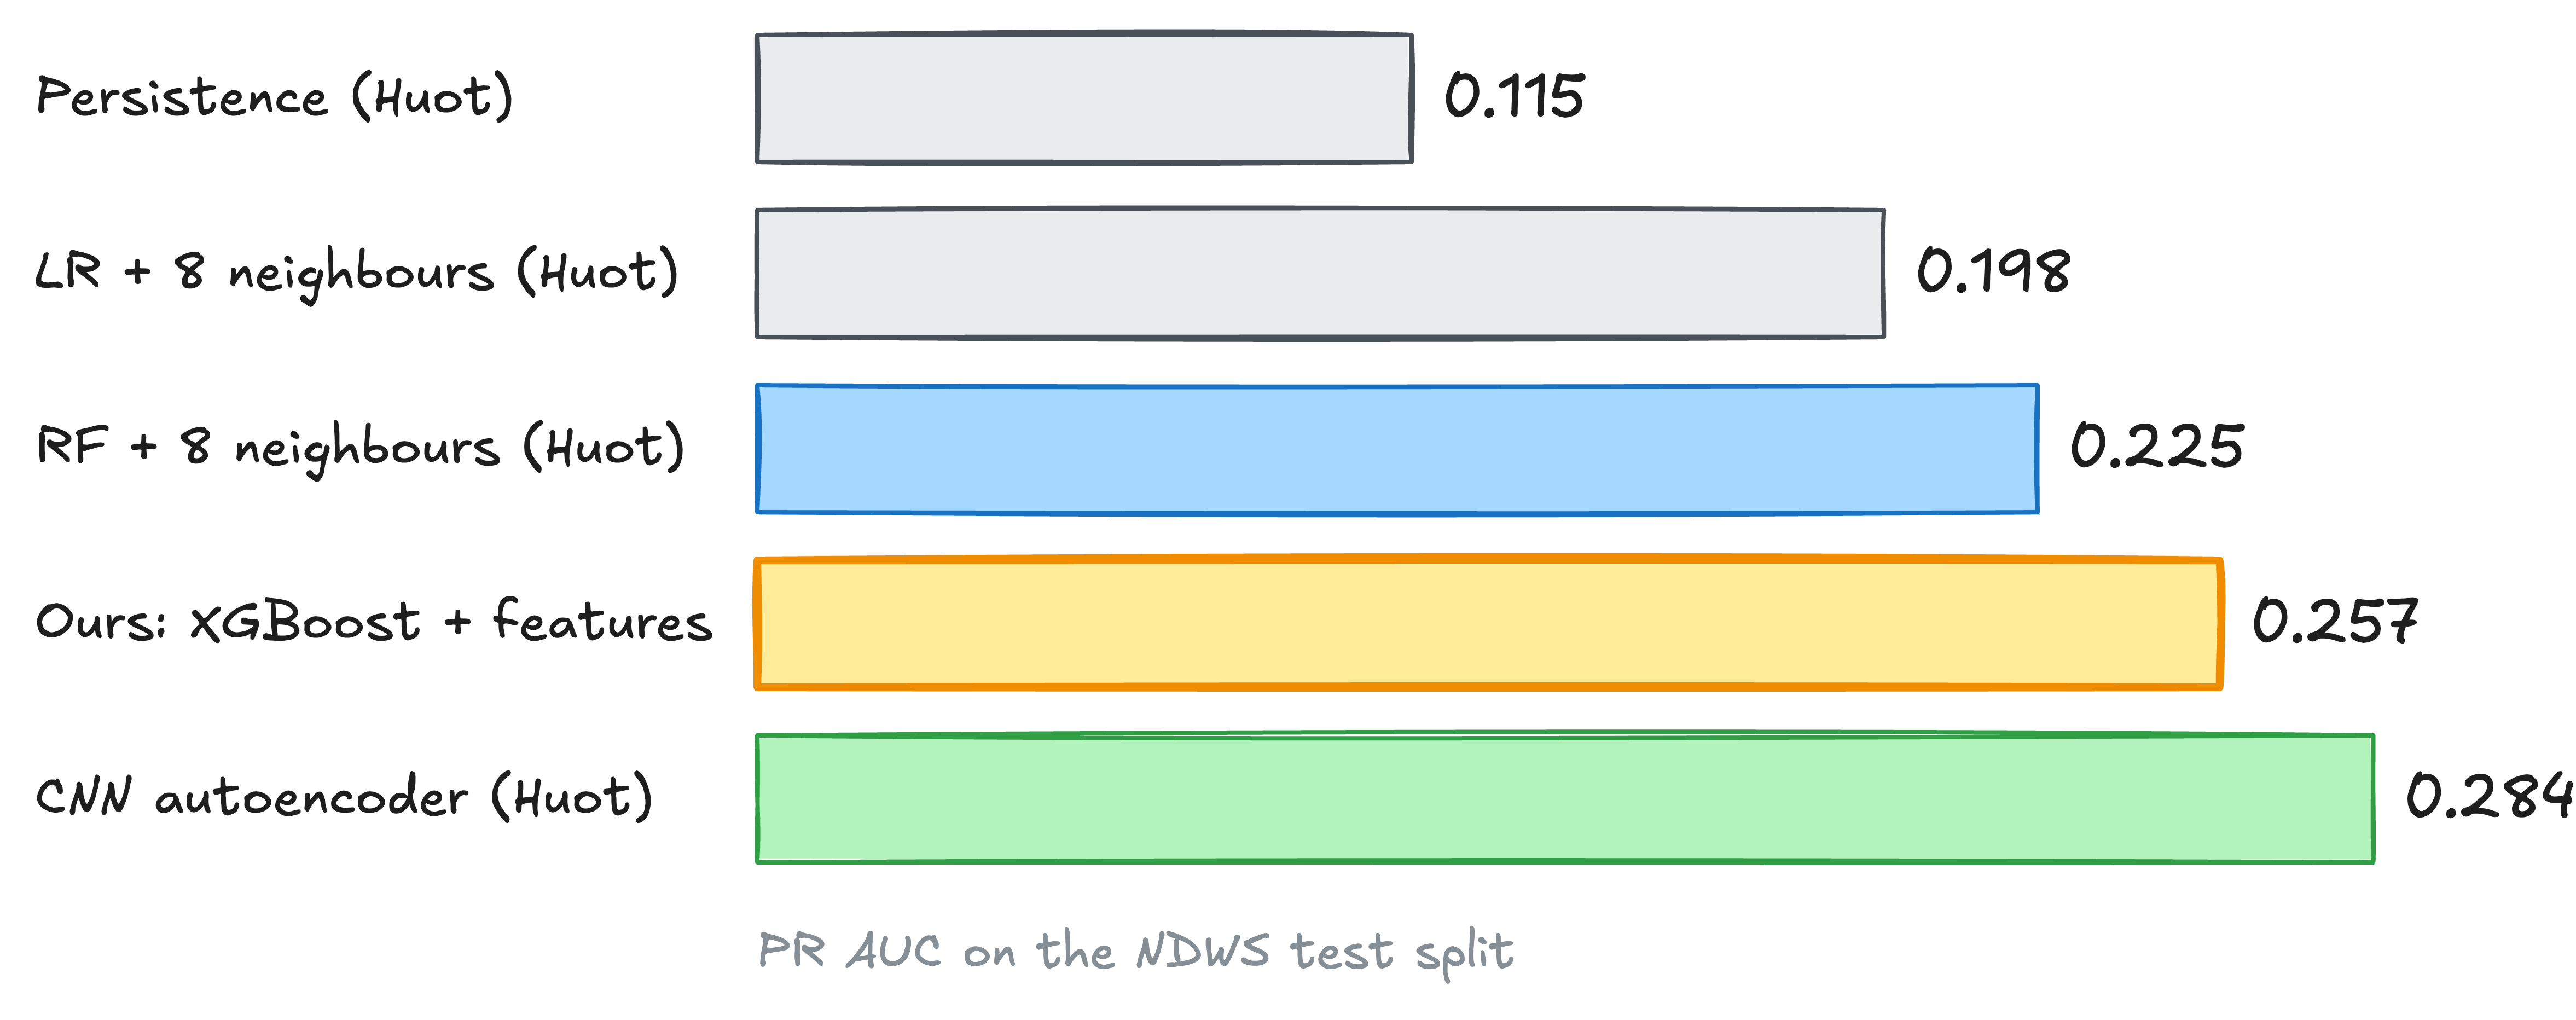
\includegraphics[width=0.66\textwidth]{slide2_where_we_stand.png}
\end{frame}

% ---------------------------------------------------------------- Sachin
\begin{frame}{What the model learned}
\begin{columns}[T]
\column{0.5\textwidth}
\footnotesize
\begin{itemize}
\item Predicts a halo around today's fire, leaning downwind
\item SHAP: fire-neighbourhood features dominate (2.29 log-odds vs 0.40 weather, 0.22 vegetation)
\item Physically sensible signs: near fire, dry air (VPD), strong wind, fire upwind $\rightarrow$ higher risk. ERC is the one exception: it acts as a proxy for region/season
\item Pushes risk downwind; train data agrees: the downwind/upwind ratio grows from 1.135 (calm) to 3.100 ($\geq$ 8\,m/s)
\end{itemize}
\src{(a) creeps outward: caught; (b) shrinking fire: false-alarm ring; (c) new fire away from the front: missed; (d) many unknown pixels. Red = hit, orange = false alarm, blue = missed.}
\column{0.46\textwidth}
\centering
\vspace{-1.6em}
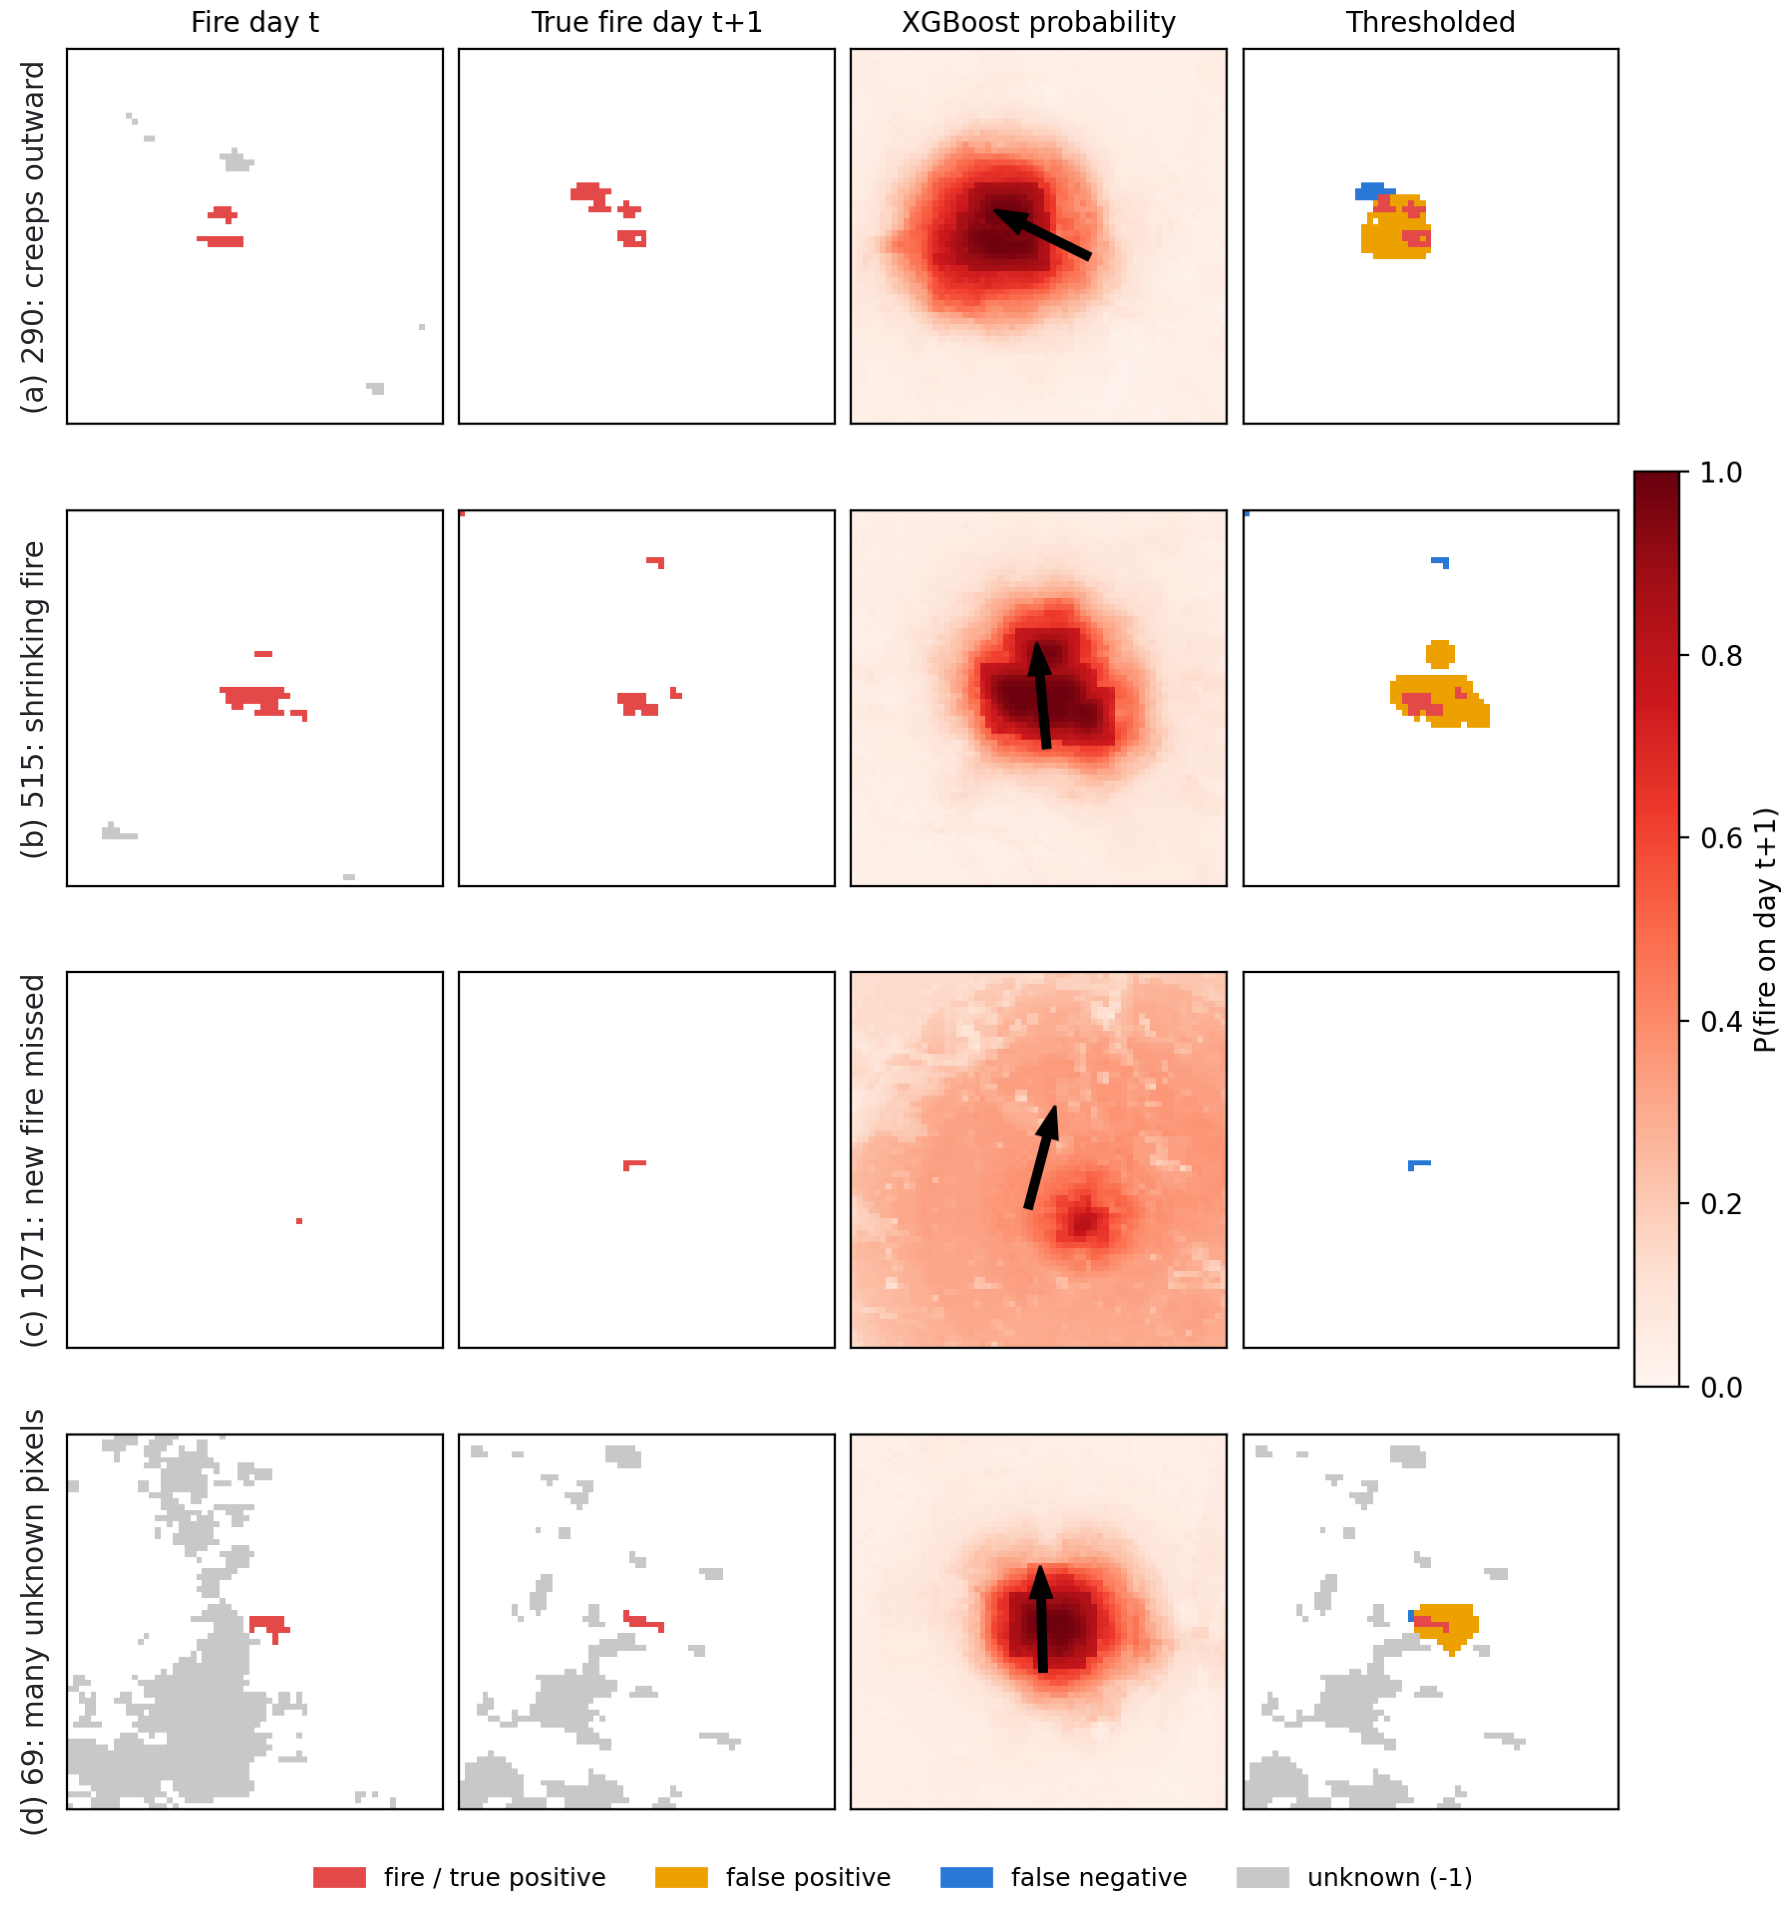
\includegraphics[height=0.78\textheight]{eval_prob_maps_selected.png}
\end{columns}
\end{frame}

% ---------------------------------------------------------------- Sachin
\begin{frame}{Where it fails}
\begin{columns}[T]
\column{0.5\textwidth}
\small
\begin{itemize}
\item False alarms around dying fires: 88.8\% within 2\,km of today's fire; only 35.3\% of burning pixels still burn tomorrow
\item Misses long-range spread: recall 0.988 at the fire, 0.648 at 2\,km, 0 beyond 5\,km (64\% of missed fire)
\item Per fire: 1\,689 test patches = only 257 fires. The ranking holds per fire (mean PR AUC 0.187 vs 0.074--0.101), but the eval threshold finds fire in only 48\% of fires vs 61\% for persistence
\item Fixed-radius halo, no fire-front shape $\rightarrow$ Phase 2
\end{itemize}
\column{0.48\textwidth}
\centering
\vspace{0.5em}
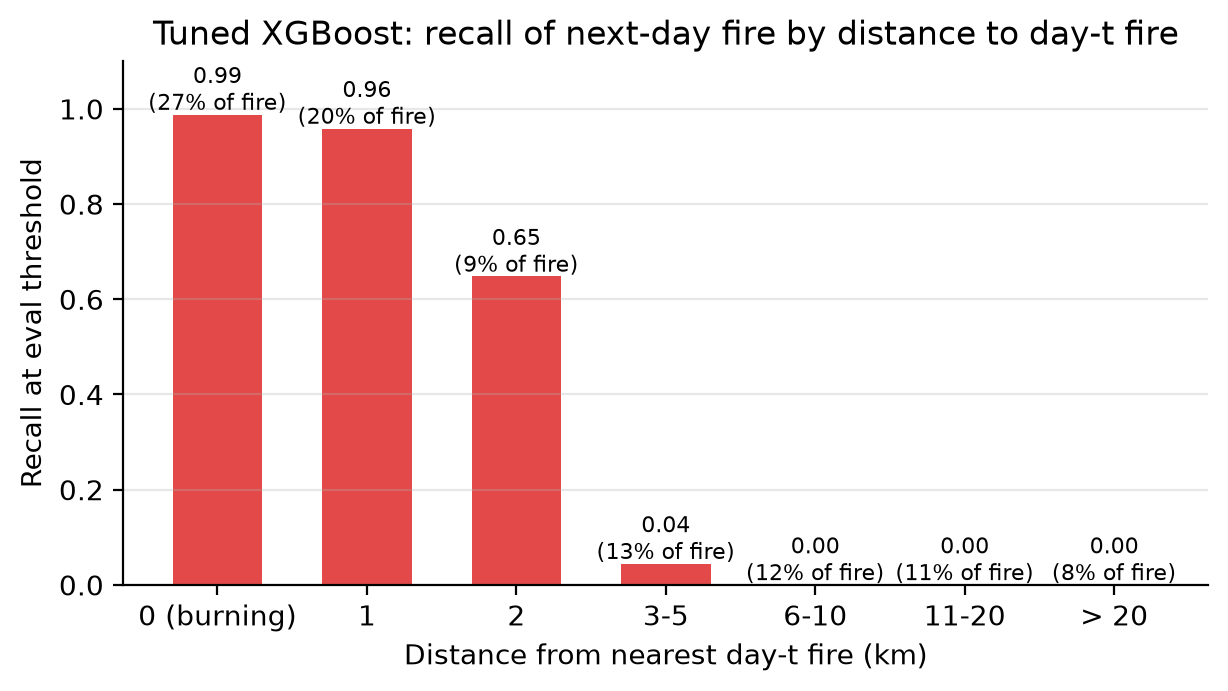
\includegraphics[width=\textwidth]{eval_recall_by_distance.png}
\end{columns}
\end{frame}

% ---------------------------------------------------------------- Priyanshu
\begin{frame}{Can we trust 0.257?}
\begin{columns}[T]
\column{0.56\textwidth}
\footnotesize
\begin{itemize}
\item Reproduced from raw TFRecords on Kaggle: every score within 0.002
\item Bootstrap over 257 fires: 0.19--0.33. Paired: XGB $>$ LGBM in 99\% of resamples, $>$ raw RF in 100\%
\item Calibration: one closed-form correction (odds $\div$ 90) gives a mean of 0.0107 vs 0.0125 observed; threshold 0.915 $\approx$ true $p$ of 0.107
\item Learning curve: 5\% of the training data $\rightarrow$ 0.204, 100\% $\rightarrow$ 0.207. Limited by bias, not variance $\rightarrow$ more data or tuning won't help
\item Location overlap: 30\% of test patches share a location with a train patch; on new locations only the ranking is unchanged (XGB 0.243 $>$ LGBM 0.234 $>$ RF 0.145 $>$ persistence 0.097)
\end{itemize}
\column{0.42\textwidth}
\centering
\vspace{1.2em}
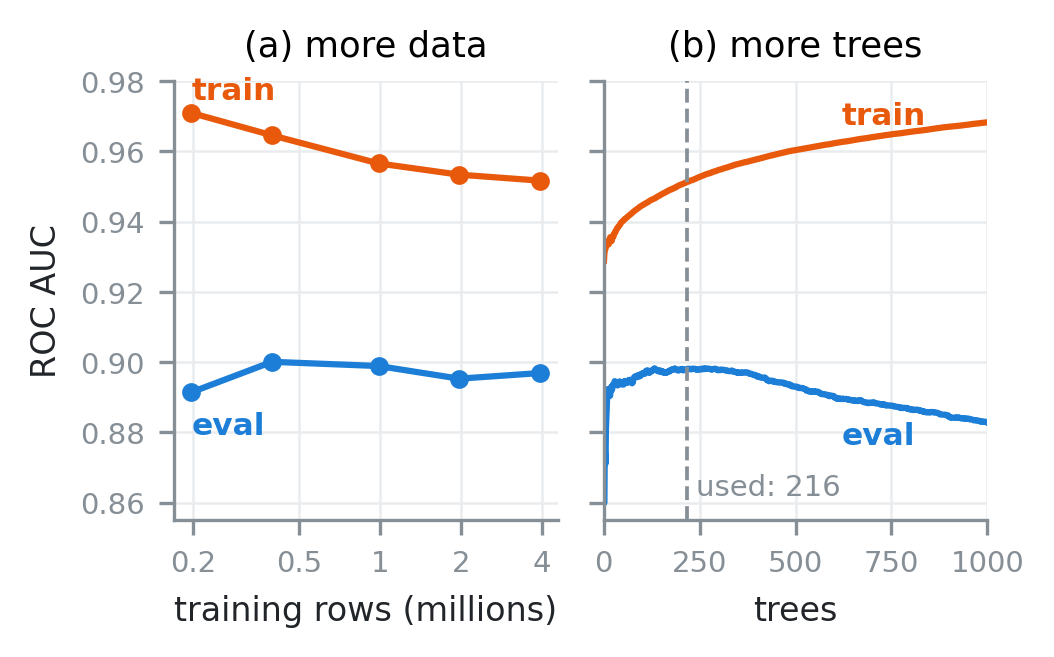
\includegraphics[width=\textwidth]{th_learning_curves.png}
\end{columns}
\end{frame}

% ---------------------------------------------------------------- Piyush
\begin{frame}{Conclusion}
\begin{itemize}
\item 23 engineered spatial features take XGBoost from 0.145 to \textbf{0.257} PR AUC (persistence 0.106), between Huot's RF and CNN
\item The signal is spatial: removing fire-neighbourhood features drops PR AUC to 0.048; tuning moves it by about 0.01
\item Robust: reproduced, holds per fire and on unseen locations, physically sensible (SHAP, downwind)
\item Limited by representation: a fixed-radius halo misses spread beyond 5\,km and over-predicts dying fires
\end{itemize}
\src{Side finding: the dataset is stored south-up, which every wind feature depends on.}
\end{frame}

% ---------------------------------------------------------------- Piyush
\begin{frame}{Future work (Phase 2)}
\begin{itemize}
\item \textbf{Whole-patch models:} U-Net / CNN that see the shape of the fire front instead of a fixed-radius halo
\item \textbf{Imbalance-aware losses:} focal loss or class-weighted segmentation loss
\item \textbf{Multi-day inputs:} fire history over several days (WildfireSpreadTS)
\item \textbf{Location-disjoint splits:} 30\% of test patches share their location with a training patch; a split that keeps locations apart would give a stricter test
\item \textbf{Uncertain labels:} better handling of cloud and smoke ($-1$) pixels than simply ignoring them
\end{itemize}
\end{frame}

% ---------------------------------------------------------------- Piyush
\begin{frame}[plain]
\centering
\vfill
{\color{accent}\Huge\bfseries Thank you\par}
\vspace{0.8em}
{\large Questions?\par}
\vspace{1.5em}
{\small\color{muted}Code, report and figures: \texttt{github.com/harshilv17/next-day-wildfire-spread}\par}
\vfill
\end{frame}

\end{document}
